\documentclass{standalone}
\usepackage{tikz}
\usepackage{ctex,siunitx}
\setCJKmainfont{Noto Serif CJK SC}
\usepackage{tkz-euclide}
\usepackage{amsmath,bbding}
\usetikzlibrary{patterns, calc}
\usetikzlibrary {decorations.pathmorphing, decorations.pathreplacing, decorations.shapes,}

\begin{document}
\small
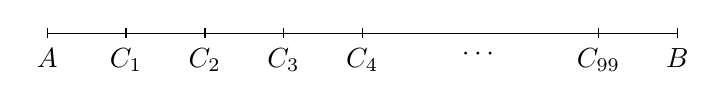
\begin{tikzpicture}[>=stealth,scale=1]
  \tkzSetUpPoint[fill=black]
  % \useasboundingbox(-0.1,-2.5)rectangle(6,3);
  \tkzDefPoints{0/0/A,8/0/B,1/0/C1,2/0/C2,3/0/C3,4/0/C4,7/0/C5,5.5/0/C6}
  \tkzDrawSegments[|-|](A,C1 C1,C2 C2,C3 C3,C4 C4,C5 C5,B)
  \tkzLabelPoints[below=2pt](A,B)
  \tkzLabelPoint[below=2pt](C1){$C_1$}
  \tkzLabelPoint[below=2pt](C2){$C_2$}
  \tkzLabelPoint[below=2pt](C3){$C_3$}
  \tkzLabelPoint[below=2pt](C4){$C_4$}
  \tkzLabelPoint[below=2pt](C5){$C_{99}$}
  \tkzLabelPoint[below=2pt](C6){$\cdots$}
\end{tikzpicture}
\end{document}